\usetikzlibrary{arrows.meta,calc}

\definecolor{orbitorange}{RGB}{230,150,20}
\definecolor{sunyellow}{RGB}{245,190,20}

\begin{figure}[H]
\centering
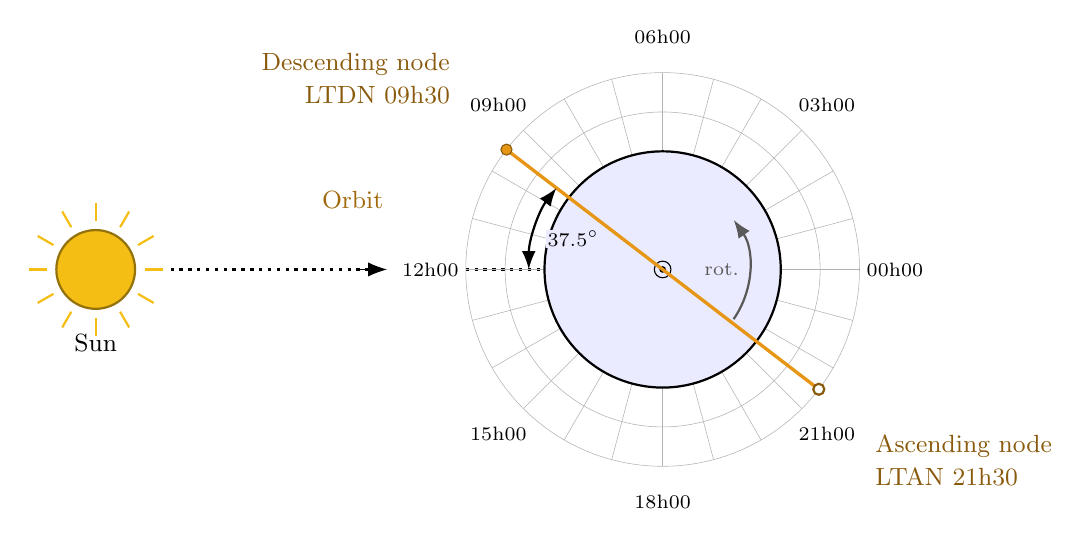
\begin{tikzpicture}[>=Latex, line join=round]

% Local solar time of a direction: angle = 15 deg * hour (noon on the Sun side, at 180 deg).
% Viewed from above the north pole the Earth rotates counter-clockwise, so local time increases counter-clockwise.

\coordinate (Ecen) at (0,0);

% ============ SUN ============
\coordinate (Sun) at (-7.2,0);
\foreach \a in {0,30,...,330}
  \draw[sunyellow, thick] ($(Sun)+(\a:0.62)$) -- ($(Sun)+(\a:0.85)$);
\filldraw[fill=sunyellow, draw=sunyellow!60!black, thick] (Sun) circle (0.5);
\node[below=20pt] at (Sun) {\small Sun};

% ============ SUN DIRECTION ============
\draw[dotted, very thick] ($(Sun)+(0.95,0)$) -- ($(Ecen)+(-3.6,0)$);
\draw[dotted, very thick] ($(Ecen)+(-2.5,0)$) -- ($(Ecen)+(-1.5,0)$);
\draw[-{Latex[length=2.4mm]}] ($(Ecen)+(-3.9,0)$) -- ($(Ecen)+(-3.5,0)$);

% ============ POLAR GRID OF LOCAL SOLAR TIME ============
% concentric rings
\foreach \r in {2.0,2.5}
  \draw[gray!60, very thin] (Ecen) circle (\r);
% hourly spokes
\foreach \a in {0,15,...,345}
  \draw[gray!60, very thin] (Ecen) -- (\a:2.5);
% labels every three hours
\foreach \h/\lab in {0/00h00, 3/03h00, 6/06h00, 9/09h00, 12/12h00, 15/15h00, 18/18h00, 21/21h00}
  \node[fill=white, inner sep=1pt] at ({15*\h}:2.95) {\scriptsize \lab};

% ============ EARTH (top view, north pole towards the viewer) ============
\filldraw[fill=blue!8, draw=black, thick] (Ecen) circle (1.5);
\fill (Ecen) circle (1.2pt);
\draw (Ecen) circle (3pt);

% direction of Earth rotation
\draw[->, thick, gray!70!black] (-35:1.1) arc (-35:35:1.1);
\node[gray!70!black, font=\scriptsize] at (0:0.75) {rot.};

% ============ ORBIT (seen edge-on from above) ============
\draw[orbitorange, very thick] (142.5:2.5) -- (322.5:2.5);
\filldraw[fill=orbitorange, draw=orbitorange!60!black] (142.5:2.5) circle (2pt);
\filldraw[fill=white, draw=orbitorange!60!black, thick] (322.5:2.5) circle (2pt);
\node[orbitorange!60!black, anchor=south east, align=right] at (142.5:3.25) {\small Descending node\\ \small LTDN 09h30};
\node[orbitorange!60!black, anchor=north west, align=left] at (322.5:3.25) {\small Ascending node\\ \small LTAN 21h30};
\node[orbitorange!70!black, anchor=north east] at (162:3.6) {\small Orbit};

% ============ LTDN ANGLE ============
\draw[<->, thick] (180:1.7) arc (180:142.5:1.7);
\node[fill=blue!8, inner sep=0.5pt] at (161:1.2) {\scriptsize $37.5^\circ$};

\end{tikzpicture}
\caption{Top view of the Earth looking down on the north pole, showing the 09h30 LTDN sun-synchronous orbit. The polar grid gives the local solar time, with noon in the direction of the Sun. The orbit is seen edge-on, with the descending node on the morning side at 09h30 and the ascending node at 21h30.}
\label{fig:ltdn_orbit}
\end{figure}
